\section{Requisiti}

Si vuole realizzare un sistema software che offra un servizio di sharing musicale, unito
alle funzionalità tipiche di un social network. Alla registrazione, l'utente dovrà
inserire una lista di generi musicali preferiti. L'algoritmo proporrà quindi all'utente i
brani più popolari basati sulle sue preferenze e gli permetterà di esplorare le sue
affinità musicali. Gli attori in gioco sono i seguenti:
\begin{itemize}
      \item utenti che vogliono ascoltare musica, conoscere e condividere le proprie
            attività musicali con gli amici;
      \item artisti indipendenti e non per pubblicare e gestire la propria musica.
\end{itemize}

L'utente, per poter usufruire dei servizi forniti, deve registrarsi e creare un proprio
profilo personale. Una volta iscritto, verrà indirizzato alla homepage che mostra i brani
più popolari dei generi preferiti dall'utente, la possibilità di cercare un brano
specifico e la sezione di impostazioni personali e social. Quando viene selezionato il
brano da scaricare, vengono fornite tutte le informazioni relative (titolo, artista,
album, anno di uscita, genere di appartenenza, numero di ascolti, durata del brano, casa
discografica).

Il software offre anche la possibilità di mettere ``like'' ai brani e di creare playlist
personalizzate. Nella propria libreria saranno quindi presenti le playlist dell'utente e
la playlist dei brani preferiti. L'interfaccia social permette invece di aggiungere gli
amici e di chattare con essi.

La funzionalità principale offerta dal servizio è l'algoritmo ``Discover'', che consente
di trovare i brani più apprezzati dalle persone che ascoltano gli stessi generi musicali
dell'utente così da permettergli di scoprire sempre nuove canzoni.

L'artista, a differenza dell'utente ascoltatore, può caricare brani singoli e album
inserendo i dati relativi alla propria produzione artistica.

L'utente, per poter usufruire dei servizi forniti, deve registrarsi e creare un proprio
profilo personale. Una volta iscritto, verrà indirizzato alla homepage che mostra i brani
più popolari dei generi preferiti dall'utente, la possibilità di cercare un brano
specifico e la sezione di impostazioni personali e social. Quando viene selezionato il
brano da scaricare, vengono fornite tutte le informazioni relative (titolo, artista,
album, anno di uscita, genere di appartenenza, numero di ascolti, durata del brano, casa
discografica).

Il software offre anche la possibilità di mettere ``like'' ai brani e di creare playlist
personalizzate. Nella propria libreria saranno quindi presenti le playlist dell'utente e
la playlist dei brani preferiti. L'interfaccia social permette invece di aggiungere gli
amici e di chattare con essi.

La funzionalità principale offerta dal servizio è l'algoritmo ``Discover'', che consente
di trovare i brani più apprezzati dalle persone che ascoltano gli stessi generi musicali
dell'utente così da permettergli di scoprire sempre nuove canzoni.

L'artista, a differenza dell'utente ascoltatore, può caricare brani singoli e album
inserendo i dati relativi alla propria produzione artistica.


\vspace{1cm}
\section{Studio di fattibilità}
Procedendo con una valutazione dei costi e dei benefici della possibile realizzazione del
presente sistema, è possibile concludere che i costi principali sono relativi alla
funzionalità di Discover e brani consigliati. 

Per realizzare questa funzionalità è
necessaria l'implementazione di un algoritmo che vada a studiare i gusti e le preferenze
di ogni singolo utente e, dopo la preliminare fase di raccolta dati, proporrà all'utente
una serie di brani in linea con le sue preferenze. 

Per quanto riguarda invece la
fattibilità in termini di tecnologie e strumenti per la realizzazione del sistema 
il costo principale da considerare è quello relativo allo sviluppo del software e il servizio di hosting sia 
della piattaforma che del database. 


\newpage
\section{Casi d'uso}
Di seguito vengono riportati i casi d'uso raggruppati in base all'attore coinvolto. Come
anticipato gli attori in gioco sono i seguenti:
\begin{itemize}
      \item Utente ascoltatore;
      \item Artista;
\end{itemize}

\subsection{Casi d'uso utente}
\begin{itemize}
      \item \textbf{UC1}: Sign in 
            
      L'utente può registrarsi inserendo le sue informazioni
            personali.
      \item \textbf{UC2}: Log in 
      
      L'utente può accedere al proprio profilo personale
            inserendo nome utente e password.
      \item \textbf{UC3}: Log out 
      
      L'utente può disconnettere il proprio profilo personale
            dal sistema.
      \item \textbf{UC4}: Consulta home-page
      
      L'utente può navigare nelle varie sezioni
            della home page.
      \item \textbf{UC5}: Cerca brano 
      
      L'utente può digitare nella barra di ricerca per cercare un brano dal titolo.
      \item \textbf{UC6}: Cerca album
      
      L'utente può digitare nella barra di ricerca per cercare un album dal titolo.
      \item \textbf{UC7}: Cerca Artista
      
      L'utente può digitare nella barra di ricerca per cercare un artista dal nome.
      
      
      \item \textbf{UC8}: Scarica brano 
      
      L'utente può scaricare il brano.
      \item \textbf{UC9}: Like al brano 
      
      L'utente può esprimere il proprio interesse per un brano mettendo like.
      \item \textbf{UC10}: Aggiungi brano a playlist
      
      L'utente può aggiungere alla lista di brani della playlist un brano selezionato.
      \item \textbf{UC11}: Cerca Utente L'utente può cercare un utente per nome dalla barra
            di ricerca apposita (cerca album/artista).
      \item \textbf{UC12}: Aggiungi Utente 
      
      L'utente può aggiungere alla propria lista amici un utente selezionato.
      \item \textbf{UC13}: Visualizza informazioni profilo 
      
      L'utente può consultare le proprie informazioni personali inserite in fase di registrazione.
      \item \textbf{UC14}: Modifica profilo 
      
      L'utente può modificare le proprie informazioni personali inserite in fase di registrazione.
      \item \textbf{UC15}: Elimina profilo 
      
      L'utente può eliminare il proprio profilo dal sistema.
      \item \textbf{UC16}: Visualizza playlist 
      
      L'utente può consultare tutte le proprie playlist.
      \item \textbf{UC17}: Crea nuova playlist L'utente può creare una nuova playlist nella
            quale aggiungere brani.
      \item \textbf{UC18}: Elimina playlist 
      
      L'utente può eliminare una delle proprie playlist.
      \item \textbf{UC19}: Modifica playlist 
      
      L'utente può modificare una delle proprie playlist, per esempio modificando il nome o rimuovendo brani.
      \item \textbf{UC20}: ``Discover'' e classifiche 
      
      L'utente può consultare classifiche e brani scelti per lui dal sistema.

\end{itemize}

\subsection{Casi d'uso artista}
\begin{itemize}
      \item \textbf{UC21}: Crea pagina artista 
      
      L'artista per poter pubblicare musica deve
            creare una pagina artista inserendo le proprie informazioni personali.
      \item  \textbf{UC22}: Visualizza pagina artista 
      
      L'artista può consultare la propria
            pagina artista, dove vengono visualizzati i propri brani/album pubblicati.
      \item  \textbf{UC23}: Aggiungi brano 
      
      L'artista può pubblicare un nuovo brano
            inserendo le informazioni relative.
      \item  \textbf{UC24}: Aggiungi album 
      
      L'artista può pubblicare un nuovo album contente
            i brani scelti.
      \item  \textbf{UC25}: Personalizza pagina artista 
      
      L'artista può decidere quali brani
            e album mettere in evidenza nella propria pagina artista.
      \item  \textbf{UC26}: Consulta anagrafica 
      
      L'artista può consultare l'anagrafica
            relativa agli ascolti e ai like dei brani e album pubblicati.

\end{itemize}


\vspace{1cm}
\subsection{Dettaglio casi d'uso}
Di seguito verranno analizzati più nel dettaglio i casi d’uso sopra citati, identificandone descrizione, attore e passi principali.

Gli utenti avranno la possibilità di registrarsi al sito per poter fruire dei servizi di streaming di musica. Al momento della registrazione sarà necessario inserire alcune informazioni personali di base come nome, cognome, email. Inoltre si dovrà inserire un nome utente identificativo e una password, necessari per il login. Nel caso in cui l’utente sia già registrato sarà necessario inserire solo questi campi per accedere al sistema. 

Al termine dell’iscrizione è possibile navigare nella Home page, la quale si suddivide in varie sezioni; ad esempio, viene offerta una selezione dei brani più ascoltati e scaricati dagli utenti. 

Una volta scelto il brano, per ognuno di essi vengono visualizzate alcune informazioni come il titolo del brano, il nome dell’artista e l’etichetta discografica di riferimento.

Alternativamente, è possibile cercare un brano dalla barra di ricerca (tramite il titolo, nome dell’artista o nome dell’album) e scaricarlo.

È offerta la possibilità di mettere like al brano e creare playlist personalizzate con i propri brani preferiti: visualizzando la propria libreria, infatti, è possibile visualizzare i Brani Preferiti e le proprie playlist. 

Come anticipato il sistema offre anche funzionalità di un social network: infatti dalla barra di ricerca è possibile cercare per nome utente i propri amici e aggiungerli, in modo tale da poter condividere le proprie preferenze musicali. 

Una delle funzionalità principali offerte dal sistema è chiamata Discover e consiste nel poter usufruire di playlist create ad hoc dal sistema per l’utente, tramite lo studio delle sue preferenze. 

Gli artisti potranno gestire e pubblicare la propria musica tramite varie funzionalità offerte dal sistema. Al momento della registrazione bisogna seguire la procedura classica di sign-in, in seguito in una sezione apposita è offerta la possibilità di creare la pagina artista, all’interno della quale verrà inserito il nome che apparirà pubblicamente, insieme ad altre informazioni personali. 

Dopo aver creato il proprio profilo artista si potrà accedere alla propria pagina per pubblicare le proprie tracce, album, playlist, personalizzandola. Ogni volta che viene pubblicato un brano è possibile inserire eventuali nomi di collaboratori, artisti che hanno partecipato al brano e scrittori di testo e musica. Ogni artista può scegliere la data dalla quale rendere accessibile il brano o l’album.







\newpage
\subsection{Diagramma dei casi d'uso}

In figura \ref{fig-uml-use-cases} è stato riportato il diagramma dei casi d'uso, dove sono stati inseriti quelli
già precedentemente descritti mettendoli in correlazione con il corrispettivo attore.

\begin{figure}[H]
      \centering
      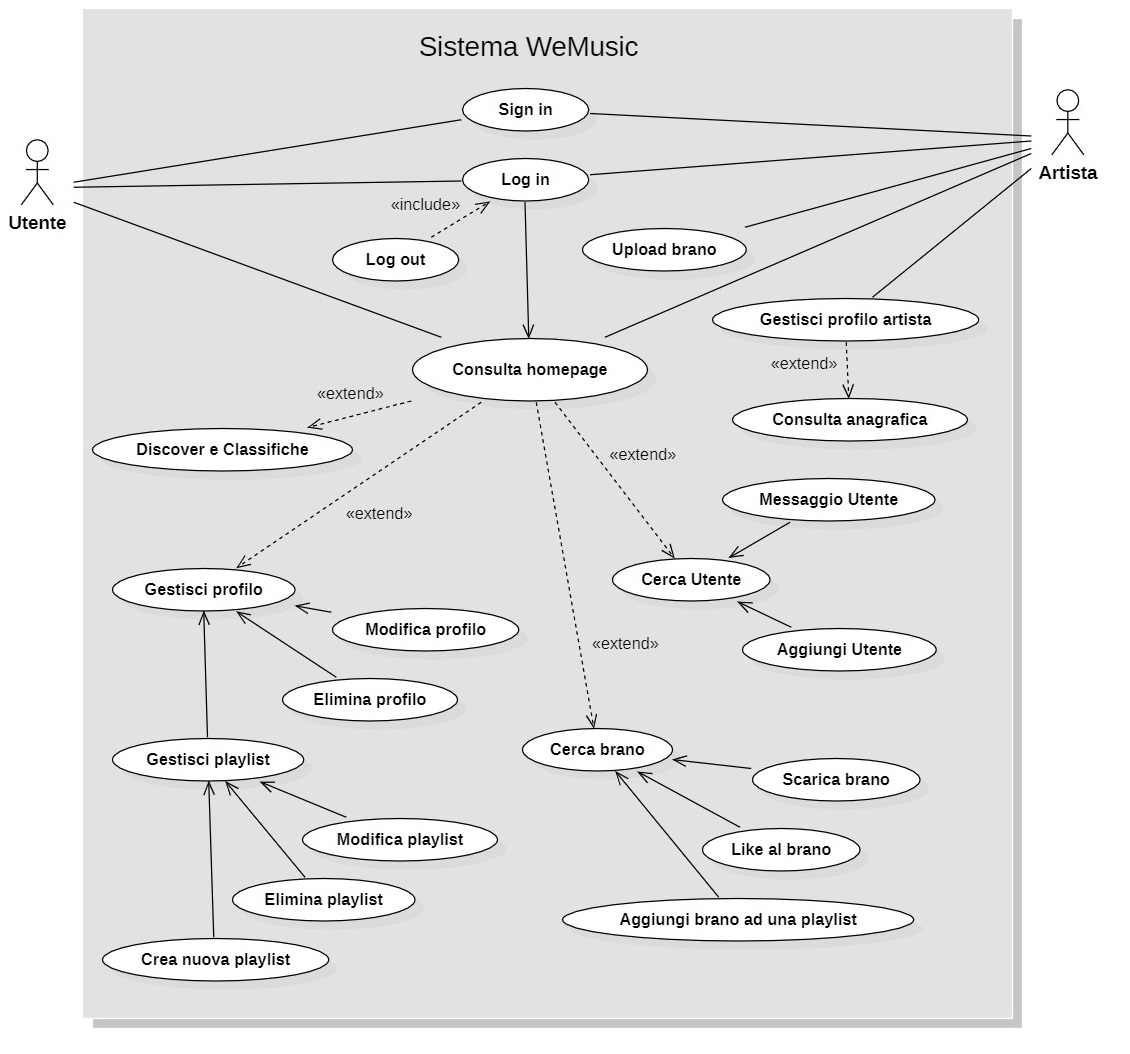
\includegraphics[scale=0.50]{UseCaseDiagramver1.jpg}
      \caption{UML use cases diagram}
      \label{fig-uml-use-cases}
\end{figure}


\newpage
\section{Architettura del sistema}
L'architettura del sistema è stata formalizzata attraverso due deployment diagram differenti: 
il primo, riportato in figura \ref{architettura}, rappresenta il sistema
attraverso una notazione a stile libero, mentre il secondo, riportato in fig (...), rappresenta
il sistema tramite lo stile UML. (...)

\subsection{Deployment diagram -- Informal}
\begin{figure}[H]
      \centering
      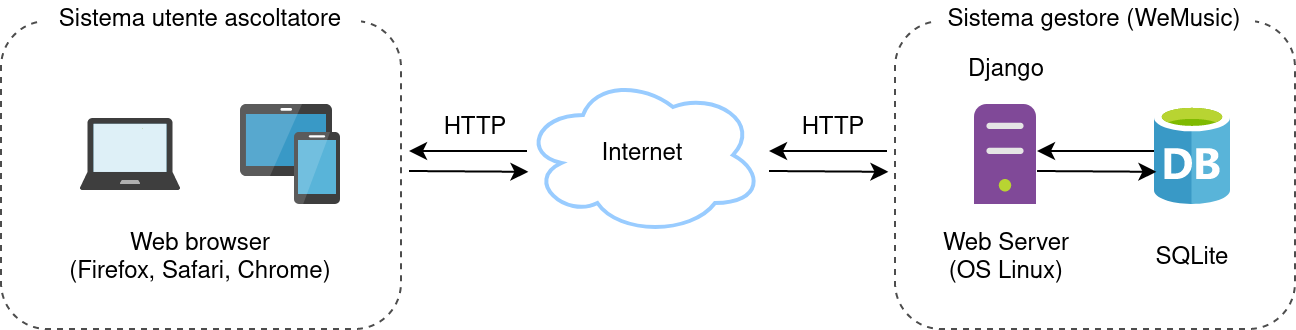
\includegraphics[width=\textwidth]{architettura.png}
      \caption{Architettura}
      \label{architettura}
\end{figure}



\subsection{Deployment diagram -- UML}

%\section{Toolchain e tecnologie utilizzate}